\documentclass{article}
\usepackage[margin=1in]{geometry}
\usepackage[outputdir=../]{minted}
\usepackage{graphicx}
\usepackage{booktabs}
\begin{document}

\title{CIS325: Medicare Part D Prescription Model}
\author{
  Christian Weber\\
  \texttt{christianweber2027@u.northwestern.edu}
}

\date{June 5th, 2025}
\maketitle

\section{Overview}

\section{Data Collection}

\section{Data Cleaning}

\section{Deploying the Neural Network Model}
Next, we deployed the Neural Network using Flask and Python. Flask provides the ability to deploy a RESTful API onto a server. Using Python, we compiled the model with keras, and exported all the labeling and preprocessing needed to serve this neural network. This was necessary as the model converts all inputs into mathematics, which is not clearly understandable for business purposes. We saved our required outputs from the jupyter notebook into both a keras-compiled model, and pickled python objects, which allow us to transfer the state of our model into a server, providing human-readable outputs for our API.

The model and application architecture is as follows:

\begin{figure}[H]
    \centering
    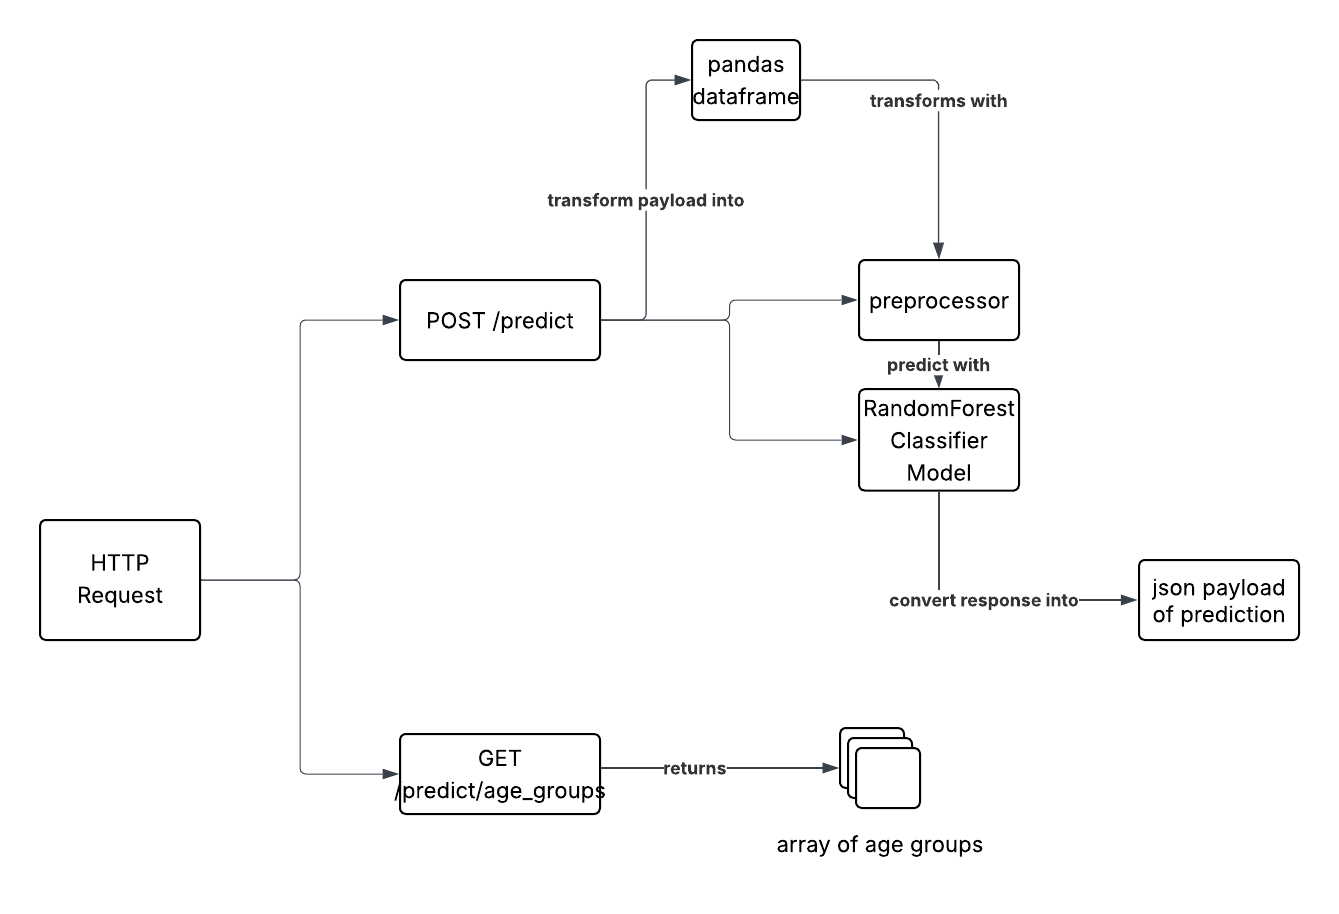
\includegraphics[width=0.75\linewidth]{paper/Code Layout-Final.png}
    \caption{Model and API Architecture}
    \label{fig:enter-label}
\end{figure}

As of publication, these endpoints are still live for testing:
\newline
\newline

\newline
\newline

\newline
\newline

To get a list of all usable practices:

\noindent\begin{minipage}{\linewidth}
\begin{minted}[fontsize=\footnotesize, breaklines, frame=single]{bash}
curl  http://ec2-54-173-183-178.compute-1.amazonaws.com/predict/practices

\end{minted}
\end{minipage}
\newline
\newline
To predict a prescription given our parameters, use curl:

\noindent\begin{minipage}{\linewidth}
\begin{minted}[fontsize=\footnotesize, breaklines, frame=single]{bash}
curl -X POST http://ec2-54-173-183-178.compute-1.amazonaws.com/predict

>{"predicted_drug":"OXYCODONE HCL"}
\end{minted}
\end{minipage}

That is to say, given a price of 5000, a supply of 30, a dermatologist may prescribe Oxycodone given our known list of prescribed narcotics.

\section{Business Value}

There is real business value to this modeling. With relative accuracy we can begin to understand prescription habits of Medicare providers whom are administering narcotics to beneficiaries under the age of 65. This gives us insights into the behaviors and incentives of medical providers and what they may be inclined to prescribe. For example, a question that can arise, but is out of scope for this research is: If all highly paid prescriptions are Oxycodone among Family Practitioners, is there a reason for that? Are drug manufacturers targeting family practitioners to such a point that we can predict how often they are likely to prescribe Oxycodone?

Other questions to consider are given the same input parameters of cost and quantity, do some practices differ in their prescription habits? If we understand statistics around our prescriptions such as standard deviation, does the model accurately predict when input parameters are out of bands?

\section{Conclusion}

In conclusion, we find that building this model was a worthwhile analysis into Medicare Part D prescription coverage. Because the dataset is 11 years old as of publication, we cannot hold this model in confidence unless we receive newer data from CMS, which appears to be unavailable. But as a point-in-time analysis, along with external research, we could begin to paint a larger puzzle on the patterns of Medicare prescriptions in the United States.

All code can be found at https://github.com/webdog/cis325-final

\section{License}
MIT License. Copyright (c) 2025 Salman Linjawi and Christian Weber.

\end{document}